\documentclass[conference]{IEEEtran}
\IEEEoverridecommandlockouts

% -------------------------------------------------------
% Packages
% -------------------------------------------------------
\usepackage[utf8]{inputenc}
\usepackage[T1]{fontenc}
\usepackage{cite}
\usepackage{amsmath,amssymb,amsfonts}
\usepackage{algorithmic}
\usepackage{graphicx}
\usepackage{textcomp}
\usepackage{xcolor}
\usepackage{booktabs}
\usepackage{multirow}
\usepackage{array}
\usepackage{url}
\usepackage{hyperref}

\hypersetup{
    colorlinks=true,
    linkcolor=blue,
    citecolor=blue,
    urlcolor=blue
}

\def\BibTeX{{\rm B\kern-.05em{\sc i\kern-.025em b}\kern-.08em
    T\kern-.1667em\lower.7ex\hbox{E}\kern-.125emX}}

% -------------------------------------------------------
\begin{document}

\title{Sleep Quality Classification: A Comparative Study\\
       Between Random Forest and MLP Neural Networks}

\author{
\IEEEauthorblockN{Cayo Murilo Pereira Figueiredo}
\IEEEauthorblockA{
  \textit{Federal University of Par\'{a} (UFPA)}\\
  Bel\'{e}m, Brazil\\
  cayomurilo09@gmail.com}
\and
\IEEEauthorblockN{Ryan Carlos Reis de Oliveira}
\IEEEauthorblockA{
  \textit{Federal University of Par\'{a} (UFPA)}\\
  Bel\'{e}m, Brazil\\
  ryan.oliveira@itec.ufpa.br}
\and
\IEEEauthorblockN{Wesley Rodrigues Heringer}
\IEEEauthorblockA{
  \textit{Federal University of Par\'{a} (UFPA)}\\
  Bel\'{e}m, Brazil\\
  wesley.heringer@itec.ufpa.br}
\and
\IEEEauthorblockN{Oscar Bruno Maciel de Abreu}
\IEEEauthorblockA{
  \textit{Federal University of Par\'{a} (UFPA)}\\
  Bel\'{e}m, Brazil\\
  oscarbma@gmail.com}
\and
\IEEEauthorblockN{Vitor Crdovil Padilha}
\IEEEauthorblockA{
  \textit{Federal University of Par\'{a} (UFPA)}\\
  Bel\'{e}m, Brazil\\
  padilha.engtelecom@gmail.com}
}


\maketitle

% -------------------------------------------------------
\begin{abstract}
This paper presents a comparative study between two supervised machine learning algorithms---Random Forest and Multilayer Perceptron (MLP) Neural Networks---applied to the binary classification of human sleep quality. The \textit{Sleep Health and Daily Performance Dataset}, a public dataset containing 100,000 records and 32 attributes relating daily habits, sleep metrics, and health indicators to the perceived recovery state (\textit{felt\_rested}), is used throughout the experiments. Both models were trained, tuned via hyperparameter optimization, and evaluated with a robust set of metrics: Accuracy, Confusion Matrix, Precision, Recall, F1-Score, ROC Curve, and AUC. Random Forest achieved superior performance, with an Accuracy of 74.15\% and a ROC AUC of 0.8218, while the optimized MLP reached 73.36\% accuracy and an AUC of 0.8145. The results indicate that tree-based models are more competitive for structured tabular data with subjective and noisy targets, particularly when predictive signal is concentrated in a small number of features.
\end{abstract}

\begin{IEEEkeywords}
Random Forest, Neural Networks, MLP, Classification, Sleep Quality, Machine Learning, Scikit-learn, TensorFlow
\end{IEEEkeywords}

% -------------------------------------------------------
\section{Introduction}

Sleep quality is a critical indicator of physical and mental health \cite{walker2017}. With the growing availability of population health data, machine learning techniques have been widely employed to model sleep patterns and predict well-being outcomes \cite{shu2020}. Among the most commonly used approaches are tree-based models such as \textit{Random Forest} \cite{breiman2001} and Artificial Neural Networks \cite{goodfellow2016}, each with distinct characteristics regarding representational capacity, computational cost, and interpretability.

This work aims to compare these two techniques on a real and relevant problem: the prediction of the variable \textit{felt\_rested}---whether an individual felt rested after a night's sleep---based on demographic, behavioral, and sleep architecture data. The choice of this problem is motivated by its clear binary nature, the richness of available attributes, and the clinical relevance of the results. The contributions of this study include a detailed exploratory analysis of the selected dataset, the implementation and hyperparameter optimization of both models, a comparative evaluation using standardized metrics, and a critical discussion of the trade-offs of each approach in practical health-related scenarios.

% -------------------------------------------------------
\section{Problem Definition and Dataset Selection}

The problem addressed is one of supervised binary classification. Given a set of descriptive attributes for an individual on a given day---sleep quality, stress level, working hours, among others---the goal is to predict whether that person felt rested upon waking ($\text{felt\_rested} = 1$) or not ($\text{felt\_rested} = 0$).

The \textit{Sleep Health and Daily Performance Dataset} was obtained from the Kaggle platform \cite{dataset2024} under a CC0 (Public Domain) license. The dataset contains 100,000 records, 32 attributes, and no missing values or duplicates, as summarized in Table~\ref{tab:dataset_info}. The target variable is slightly imbalanced: the majority class (not rested) accounts for 60.99\% of records, while the positive class (rested) represents the remaining 39.01\%.

\begin{table}[!ht]
\caption{Dataset Characteristics}
\label{tab:dataset_info}
\centering
\begin{tabular}{ll}
\toprule
\textbf{Property} & \textbf{Value} \\
\midrule
Total records         & 100,000 \\
Total attributes      & 32 \\
Missing values        & 0 \\
Duplicate records     & 0 \\
Target variable       & \texttt{felt\_rested} (binary) \\
Class 0 (not rested)  & 60,988 (60.99\%) \\
Class 1 (rested)      & 39,012 (39.01\%) \\
CSV file size         & 14.3 MB \\
\bottomrule
\end{tabular}
\end{table}

The dataset is synthetic, calibrated based on real epidemiological studies (CDC, Sleep Foundation, Framingham Heart Study), which ensures clinically plausible correlations. Among the main correlations reported by the author are: stress vs.\ sleep quality ($r = -0.64$), REM sleep percentage vs.\ cognitive performance ($r = +0.45$), and age vs.\ deep sleep ($r = -0.45$). The 32 attributes are organized into functional groups covering demographic data (\texttt{age}, \texttt{gender}, \texttt{occupation}, \texttt{bmi}), sleep architecture (\texttt{sleep\_duration\_hrs}, \texttt{sleep\_quality\_score}, \texttt{rem\_percentage}, \texttt{deep\_sleep\_percentage}), lifestyle (\texttt{caffeine\_intake\_mg}, \texttt{exercise\_day}, \texttt{steps\_that\_day}), psychological and occupational factors (\texttt{stress\_score}, \texttt{work\_hours\_that\_day}), and health context (\texttt{heart\_rate\_resting\_bpm}, \texttt{shift\_work}, \texttt{room\_temperature\_celsius}).

The dataset was selected because it fully meets the requirements of this work: sufficient volume to train neural networks (100k records), no missing values, a clear binary target variable, and mixed attributes (numerical and categorical) that allow for a comprehensive demonstration of preprocessing techniques. The mild class imbalance is moderate enough to be handled with stratified splitting and critical metric analysis, without requiring advanced resampling techniques.

% -------------------------------------------------------
\section{Data Preprocessing}

\subsection{Exploratory Data Analysis (EDA)}

The exploratory analysis revealed relevant patterns for modeling. Regarding the target distribution, the majority class ($\text{felt\_rested} = 0$) represents 60.99\% of records, meaning a naive classifier would achieve approximately 61\% accuracy without learning any real pattern---which justifies the use of complementary metrics such as F1-Score, Balanced Accuracy, and ROC AUC.

In terms of correlations with the target, the variables \texttt{sleep\_quality\_score} ($r = +0.48$) and \texttt{sleep\_duration\_hrs} ($r = +0.42$) showed the strongest positive correlations with \texttt{felt\_rested}. The \texttt{stress\_score} exhibited a moderate negative correlation ($r = -0.37$), and \texttt{work\_hours\_that\_day} was also negatively correlated ($r = -0.28$). These relationships are visually summarized in the correlation heatmap shown in Figure~\ref{fig:heatmap}, which confirms that sleep duration and quality are by far the most linearly associated variables with the target, while demographic features such as age and BMI contribute only marginally. The variable \texttt{occupation} also revealed substantial differences in the perceived rest rate among professional groups, with occupations involving heavier nocturnal or irregular workloads showing lower rates of $\texttt{felt\_rested} = 1$.

\begin{figure}[!ht]
\centering
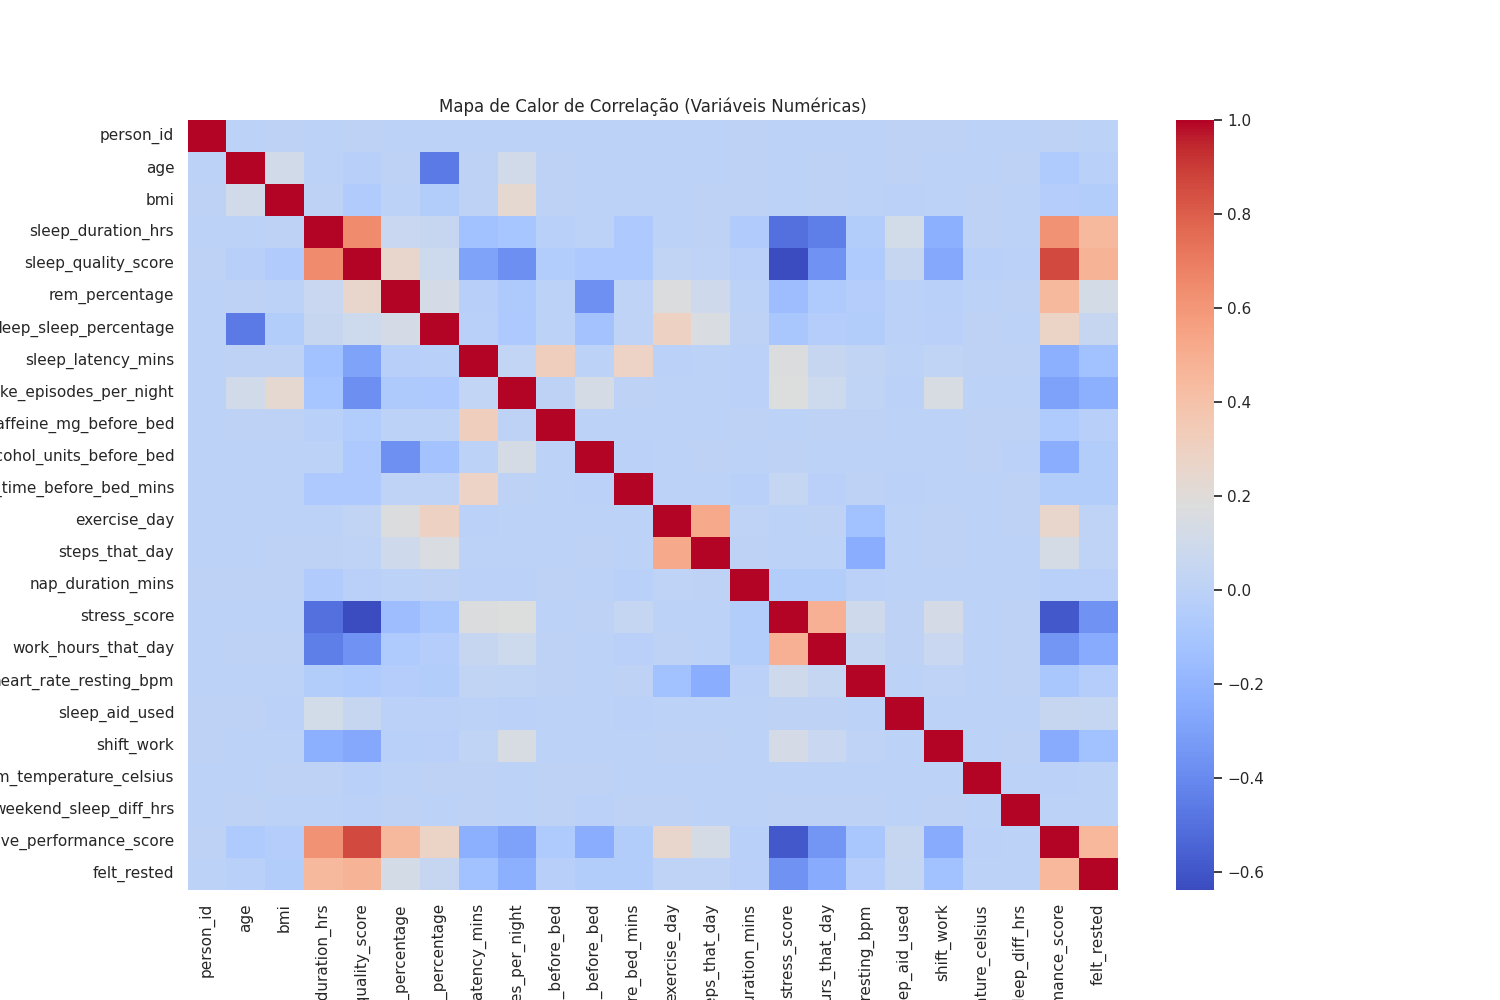
\includegraphics[width=\columnwidth]{correlation_heatmap.png}
\caption{Correlation heatmap for the numerical variables in the dataset. The strongest associations with the target variable \texttt{felt\_rested} are observed for \texttt{sleep\_quality\_score}, \texttt{sleep\_duration\_hrs}, and \texttt{stress\_score}.}
\label{fig:heatmap}
\end{figure}

The analysis of boxplots across the sleep architecture variables, shown in Figure~\ref{fig:boxplot}, further confirms these findings. Individuals with $\texttt{felt\_rested} = 1$ present significantly higher distributions in \texttt{sleep\_duration\_hrs} and \texttt{sleep\_quality\_score}, with a median sleep duration roughly one hour greater than the non-rested group. The REM sleep percentage also shows a modest but consistent upward shift for the rested class, while deep sleep percentage remains nearly indistinguishable between the two groups---suggesting that total duration and subjective quality are more predictive than specific sleep stage composition.

\begin{figure}[!ht]
\centering
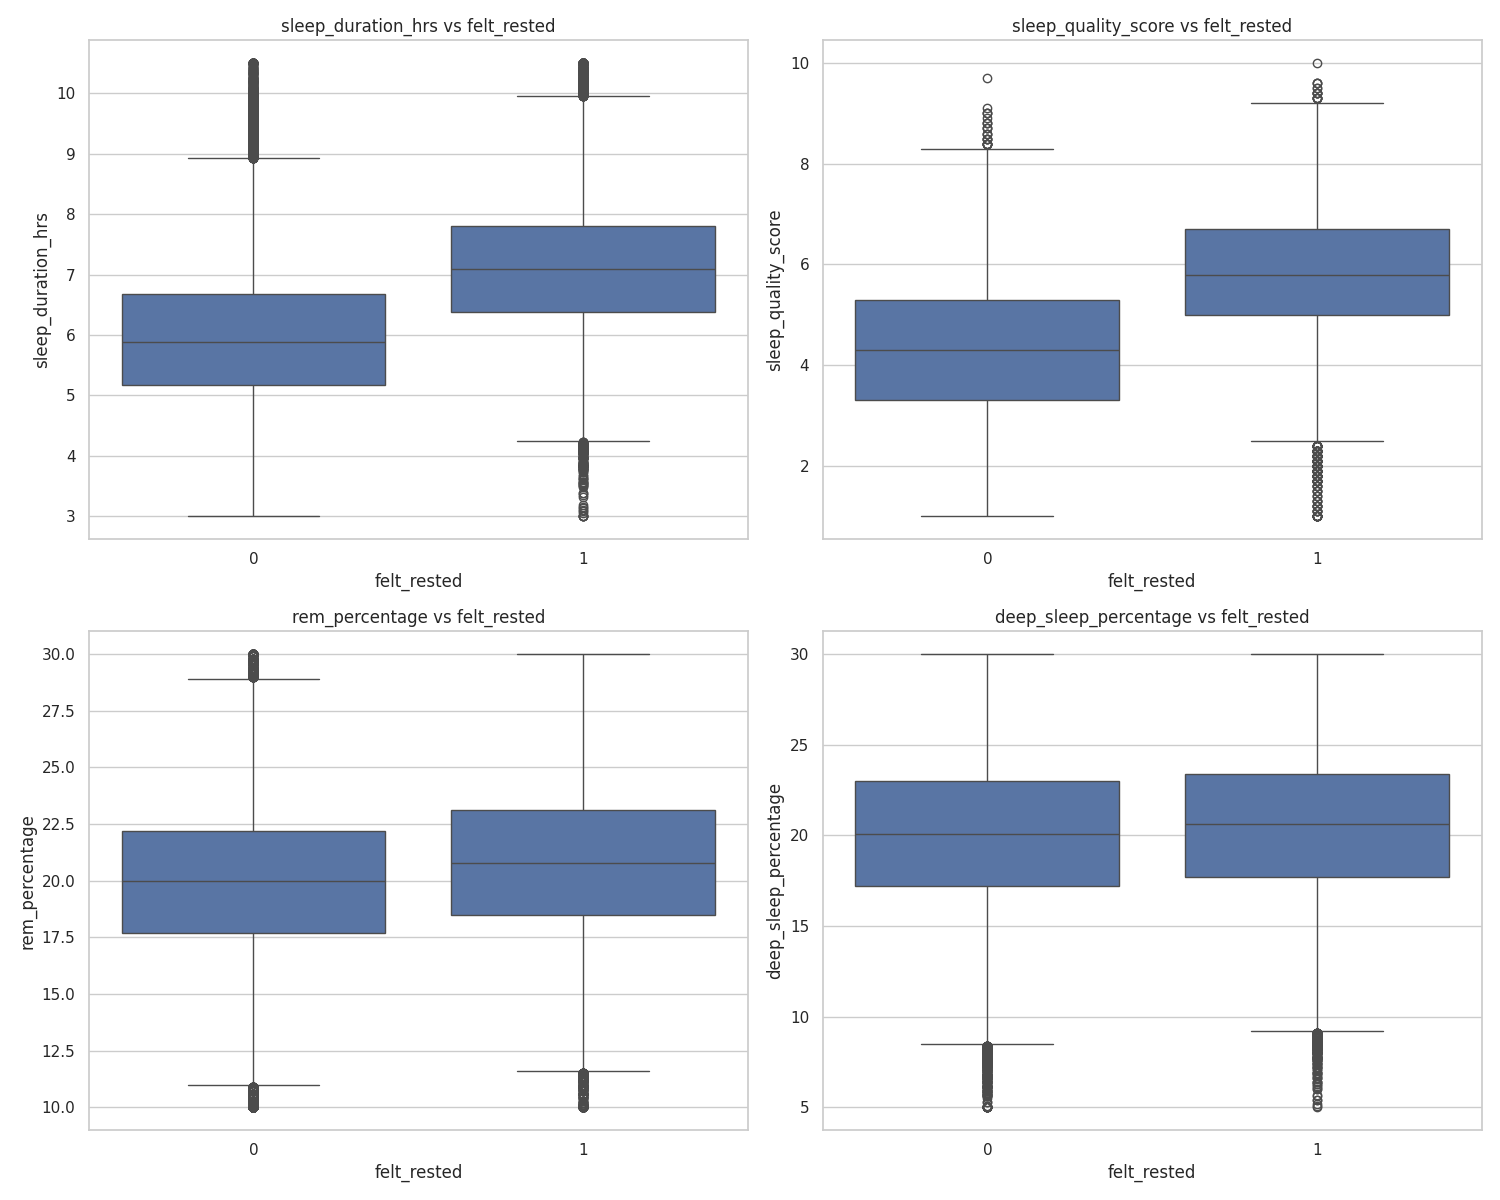
\includegraphics[width=\columnwidth]{sleep_features_boxplot.png}
\caption{Distribution of the main sleep architecture variables segmented by the target class \texttt{felt\_rested}. Individuals in class 1 (rested) show notably higher sleep duration and quality scores, while deep sleep percentage presents minimal separation between groups.}
\label{fig:boxplot}
\end{figure}

\subsection{Preprocessing Techniques}

The preprocessing pipeline was implemented using Scikit-learn's \texttt{ColumnTransformer} \cite{sklearn2011} to ensure reproducibility and prevent data leakage. Numerical variables were normalized via Z-score standardization (\texttt{StandardScaler}), transforming each attribute to zero mean and unit standard deviation---necessary to stabilize the gradient of the neural network and ensure comparability in distance-based metrics. Categorical variables were encoded using One-Hot Encoding (\texttt{OneHotEncoder} with \texttt{handle\_unknown='ignore'}), avoiding spurious ordinal relationships between categories. No null value treatment was required, as the dataset contains none. The column \texttt{person\_id} was dropped for containing no predictive information, and the columns \texttt{sleep\_disorder\_risk} and \texttt{cognitive\_performance\_score} were excluded as they are alternative target variables whose inclusion would cause data leakage.

\subsection{Data Splitting}

The dataset was split into 80\% for training (80,000 samples) and 20\% for testing (20,000 samples), with stratification by the target variable to preserve the original class proportions in both sets. The \texttt{random\_state=42} was fixed to ensure reproducibility. The same split was used for all models, ensuring a fair comparison of results.

\subsection{Feature Engineering (MLP v2)}

For the optimized version of the neural network, three interaction features were created based on clinical hypotheses. The first, \texttt{stress\_work\_interaction} $= \text{stress\_score} \times \text{work\_hours\_that\_day}$, captures the combined effect of stress and work overload. The second, \texttt{sleep\_efficiency} $= (\text{rem\_percentage} + \text{deep\_sleep\_percentage}) / 100$, summarizes the proportion of restorative sleep. The third, \texttt{age\_stress\_ratio} $= \text{stress\_score} / (\text{age} + 1)$, models the interaction between stress and aging.

% -------------------------------------------------------
\section{Implementation and Training}

\subsection{Random Forest}

Random Forest was implemented using Scikit-learn's \texttt{RandomForestClassifier}, wrapped in a \texttt{Pipeline} that combines preprocessing and the classifier. Hyperparameter search was performed with \texttt{GridSearchCV} using 3-fold cross-validation, with F1-Score as the selection criterion. The search space covered the combinations described in Table~\ref{tab:rf_grid}, and the best hyperparameters found were \texttt{n\_estimators = 200}, \texttt{max\_depth = 20}, and \texttt{min\_samples\_split = 2}.

\begin{table}[!ht]
\caption{Hyperparameter Grid --- Random Forest}
\label{tab:rf_grid}
\centering
\begin{tabular}{ll}
\toprule
\textbf{Hyperparameter} & \textbf{Tested Values} \\
\midrule
\texttt{n\_estimators}      & \{100, 200\} \\
\texttt{max\_depth}          & \{None, 10, 20\} \\
\texttt{min\_samples\_split} & \{2, 5\} \\
\bottomrule
\end{tabular}
\end{table}

\subsection{MLP Neural Network --- Baseline Version}

The first version of the neural network (baseline) was implemented with TensorFlow/Keras \cite{chollet2015}, with the architecture described in Table~\ref{tab:mlp_baseline}. The model was compiled with the Adam optimizer, binary cross-entropy loss function, and an EarlyStopping callback with a patience of 10 epochs monitoring validation loss.

\begin{table}[!ht]
\caption{Baseline MLP Neural Network Architecture}
\label{tab:mlp_baseline}
\centering
\begin{tabular}{llll}
\toprule
\textbf{Layer} & \textbf{Neurons} & \textbf{Activation} & \textbf{Regularization} \\
\midrule
Dense 1  & 64  & ReLU    & Dropout(0.2) \\
Dense 2  & 32  & ReLU    & Dropout(0.1) \\
Dense 3  & 16  & ReLU    & --- \\
Output   & 1   & Sigmoid & --- \\
\bottomrule
\end{tabular}
\end{table}

\subsection{MLP Neural Network --- Optimized Version}

The second version (v2) incorporated several optimization techniques over the baseline. The network capacity was increased to 128 neurons in the first dense layer, and \texttt{BatchNormalization} was inserted after each layer to stabilize the gradient and accelerate convergence. A \texttt{ReduceLROnPlateau} callback was added to reduce the learning rate by a factor of 0.5 when validation loss stagnated for 5 consecutive epochs, and the epoch limit was raised to 100 with EarlyStopping patience of 12. The resulting architecture is described in Table~\ref{tab:mlp_v2}.

\begin{table}[!ht]
\caption{Optimized MLP Neural Network Architecture (v2)}
\label{tab:mlp_v2}
\centering
\begin{tabular}{llll}
\toprule
\textbf{Layer} & \textbf{Neurons} & \textbf{Activation} & \textbf{Regularization} \\
\midrule
Dense 1  & 128 & ReLU    & BatchNorm + Dropout(0.3) \\
Dense 2  & 64  & ReLU    & BatchNorm + Dropout(0.2) \\
Dense 3  & 32  & ReLU    & BatchNorm \\
Dense 4  & 16  & ReLU    & --- \\
Output   & 1   & Sigmoid & --- \\
\bottomrule
\end{tabular}
\end{table}

% -------------------------------------------------------
\section{Results}

Table~\ref{tab:results_main} presents the full performance comparison between the models on the test set (20,000 samples). Random Forest stood out across virtually all evaluated metrics, while both MLP versions performed similarly to each other, with the optimized version achieving only a marginal gain over the baseline.

\begin{table}[!ht]
\caption{Performance Comparison on the Test Set}
\label{tab:results_main}
\centering
\renewcommand{\arraystretch}{1.3}
\begin{tabular}{lccc}
\toprule
\textbf{Metric} & \textbf{RF} & \textbf{MLP v1} & \textbf{MLP v2} \\
\midrule
Accuracy            & \textbf{74.15\%} & 73.23\% & 73.36\% \\
Balanced Accuracy   & \textbf{73.09\%} & ---     & ---     \\
Precision (cl. 1)   & \textbf{65.28\%} & 63.00\% & 64.00\% \\
Recall (cl. 1)      & 69.99\%          & 64.00\% & \textbf{65.00\%} \\
F1-Score (cl. 1)    & \textbf{67.56\%} & 64.00\% & 65.00\% \\
ROC AUC             & \textbf{0.8218}  & 0.8142  & 0.8145  \\
\bottomrule
\multicolumn{4}{l}{\footnotesize RF = Random Forest; MLP v1 = Baseline; MLP v2 = Optimized} \\
\end{tabular}
\end{table}

As a minimum reference point, the naive classifier (always predicting the majority class) achieved Accuracy = 60.99\%, F1 = 0.00, and ROC AUC = 0.50. Both models consistently surpass this baseline, with gains of approximately 13 percentage points in accuracy and 0.32 in AUC.

Table~\ref{tab:confusion} details the confusion matrix of the Random Forest, the best-performing model. Of the 7,802 real positive-class samples in the test set, the model correctly identified 5,461 (Recall = 69.99\%). The 2,904 False Positives represent cases where the model predicted rest when the individual did not feel rested---the most harmful type of error in health screening contexts, as it may mask real sleep problems.

\begin{table}[!ht]
\caption{Confusion Matrix --- Random Forest (Test Set)}
\label{tab:confusion}
\centering
\renewcommand{\arraystretch}{1.3}
\begin{tabular}{llcc}
\toprule
 & & \multicolumn{2}{c}{\textbf{Predicted}} \\
\cmidrule(lr){3-4}
 & & \textbf{Class 0} & \textbf{Class 1} \\
\midrule
\multirow{2}{*}{\textbf{Actual}} & \textbf{Class 0} & 9,294 (TN) & 2,904 (FP) \\
                                  & \textbf{Class 1} & 2,341 (FN) & 5,461 (TP) \\
\bottomrule
\end{tabular}
\end{table}

Figure~\ref{fig:roc} illustrates the ROC curves for all three models. The AUC of 0.82 indicates good discriminative capacity between rested and non-rested individuals: in practical terms, there is an 82\% probability that the model will rank a rested individual with a higher score than a non-rested one, chosen at random. The gap between Random Forest and both MLP versions is consistent across all classification thresholds, reinforcing that the advantage is not an artifact of a particular operating point.

\begin{figure}[!ht]
\centering
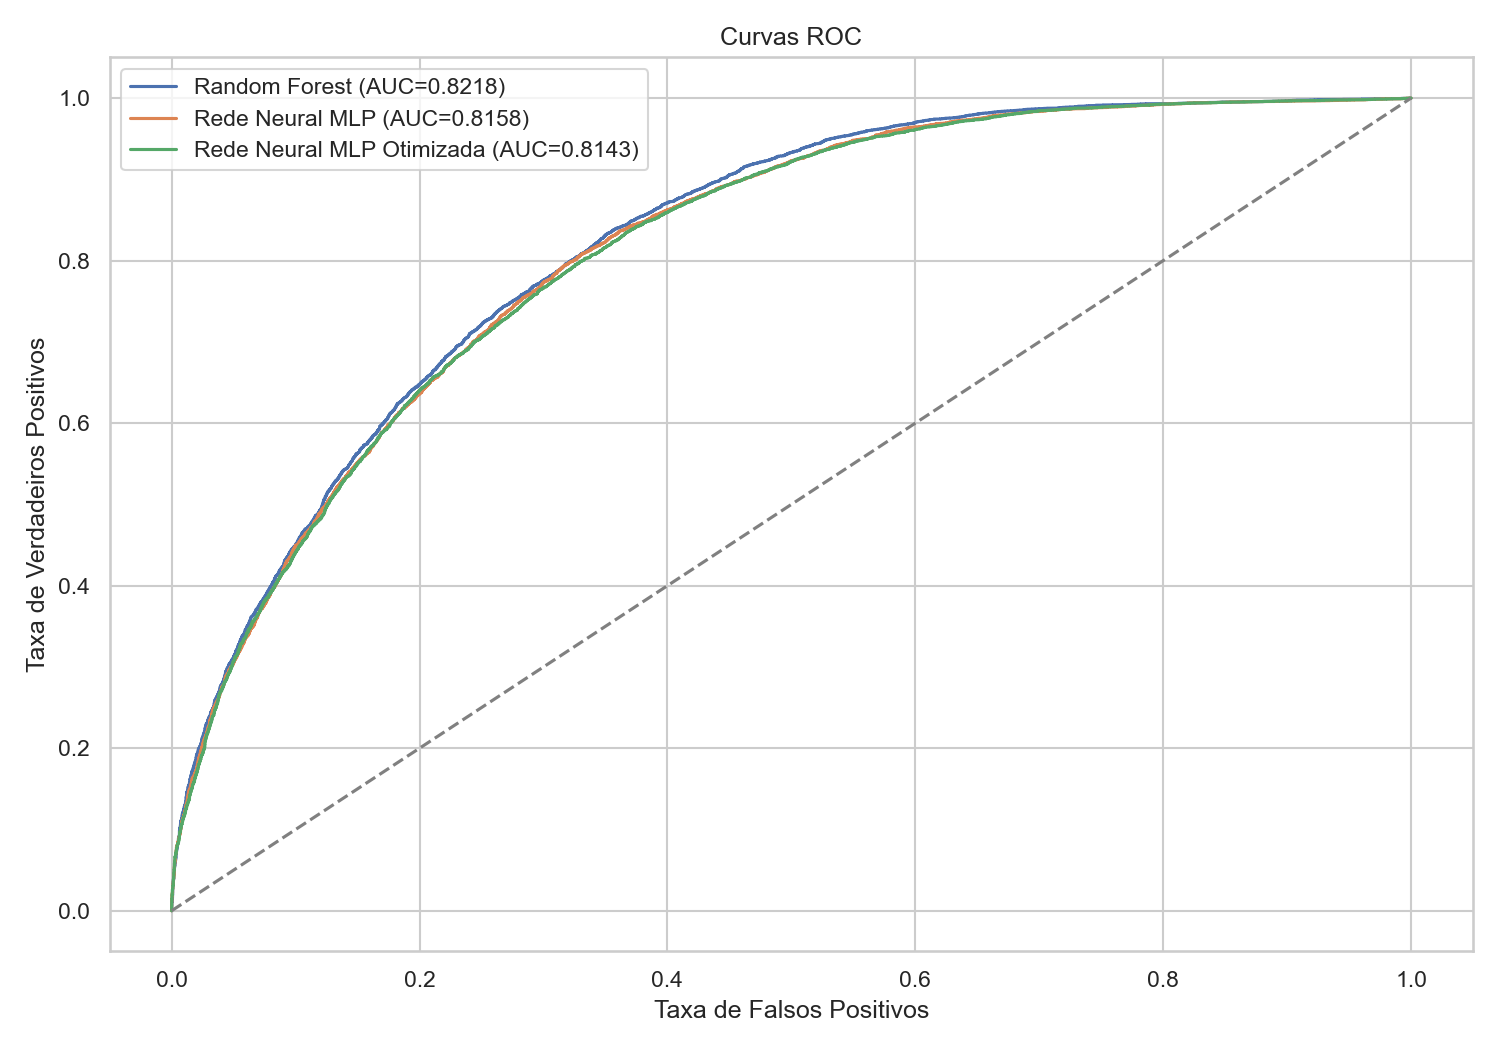
\includegraphics[width=\columnwidth]{roc_curves.png}
\caption{Comparative ROC curves for the three evaluated models. Random Forest (AUC = 0.8218) exhibits superior discriminative capacity over the MLP across all classification thresholds.}
\label{fig:roc}
\end{figure}

The permutation importance analysis, summarized in Table~\ref{tab:feature_imp}, revealed that predictive signal is strongly concentrated in a small number of variables. The variable \texttt{sleep\_duration\_hrs} is by far the most important predictor (an AUC drop of 11.65 p.p.\ when permuted), followed by \texttt{sleep\_quality\_score} (4.20 p.p.). The remaining variables contribute marginally (each causing less than 0.003 AUC drop), indicating that the problem has few truly informative dimensions.

\begin{table}[!ht]
\caption{Permutation Importance --- Random Forest (Top 5)}
\label{tab:feature_imp}
\centering
\begin{tabular}{lcc}
\toprule
\textbf{Feature} & \textbf{AUC Drop} & \textbf{SD} \\
\midrule
\texttt{sleep\_duration\_hrs}      & 0.1165 & 0.0048 \\
\texttt{sleep\_quality\_score}     & 0.0420 & 0.0031 \\
\texttt{wake\_episodes\_per\_night}& 0.0211 & 0.0030 \\
\texttt{stress\_score}             & 0.0172 & 0.0022 \\
\texttt{day\_type}                 & 0.0017 & 0.0004 \\
\bottomrule
\end{tabular}
\end{table}

Finally, a decision threshold sweep demonstrated that the default value of 0.50 is not necessarily optimal for this problem. A threshold of 0.35 maximizes F1 (0.7017) and Recall (0.8491) at the cost of lower Accuracy (71.84\%), while a threshold of 0.39 maximizes Balanced Accuracy (74.24\%). This result highlights the importance of tuning the decision threshold according to the costs associated with each type of error in the application domain.

% -------------------------------------------------------
\section{Evaluation}

Considering the results as a whole, Random Forest proved consistently superior to the MLP Neural Network across all main metrics, with an advantage of 0.79 p.p.\ in Accuracy, 2.56 p.p.\ in F1-Score, and 0.0073 in ROC AUC relative to the best MLP version. Although the absolute differences are modest, their consistency across all metrics is not trivial---it reflects structural characteristics of the problem that intrinsically favor tree-based models. Figure~\ref{fig:model_comparison} provides a visual synthesis of this comparison, making clear that the Random Forest's lead is uniform rather than isolated to a single metric. Tabular data with mixed attributes is the natural domain of Random Forest: decision trees capture non-linear interactions without the need for explicit feature engineering, and the bagging ensemble reduces variance without incurring the cost of gradient optimization. Recent literature corroborates this observation \cite{grinsztajn2022}, noting that tree-based models outperform neural networks on tabular benchmarks precisely because predictive signal tends to be concentrated in a few variables---exactly what the permutation importance analysis confirmed in this experiment, with \texttt{sleep\_duration\_hrs} alone accounting for an 11.65 p.p.\ AUC drop. With only four variables driving virtually all predictive power, the distributed representational capacity that is the theoretical advantage of neural networks simply has no room to exercise itself. Added to this, the subjective nature of the \texttt{felt\_rested} variable---a self-assessment in which two individuals with objectively identical sleep profiles may respond differently---introduces irreducible noise into the data that limits the predictability ceiling of the problem and penalizes models with greater memorization capacity more heavily.

\begin{figure}[!ht]
\centering
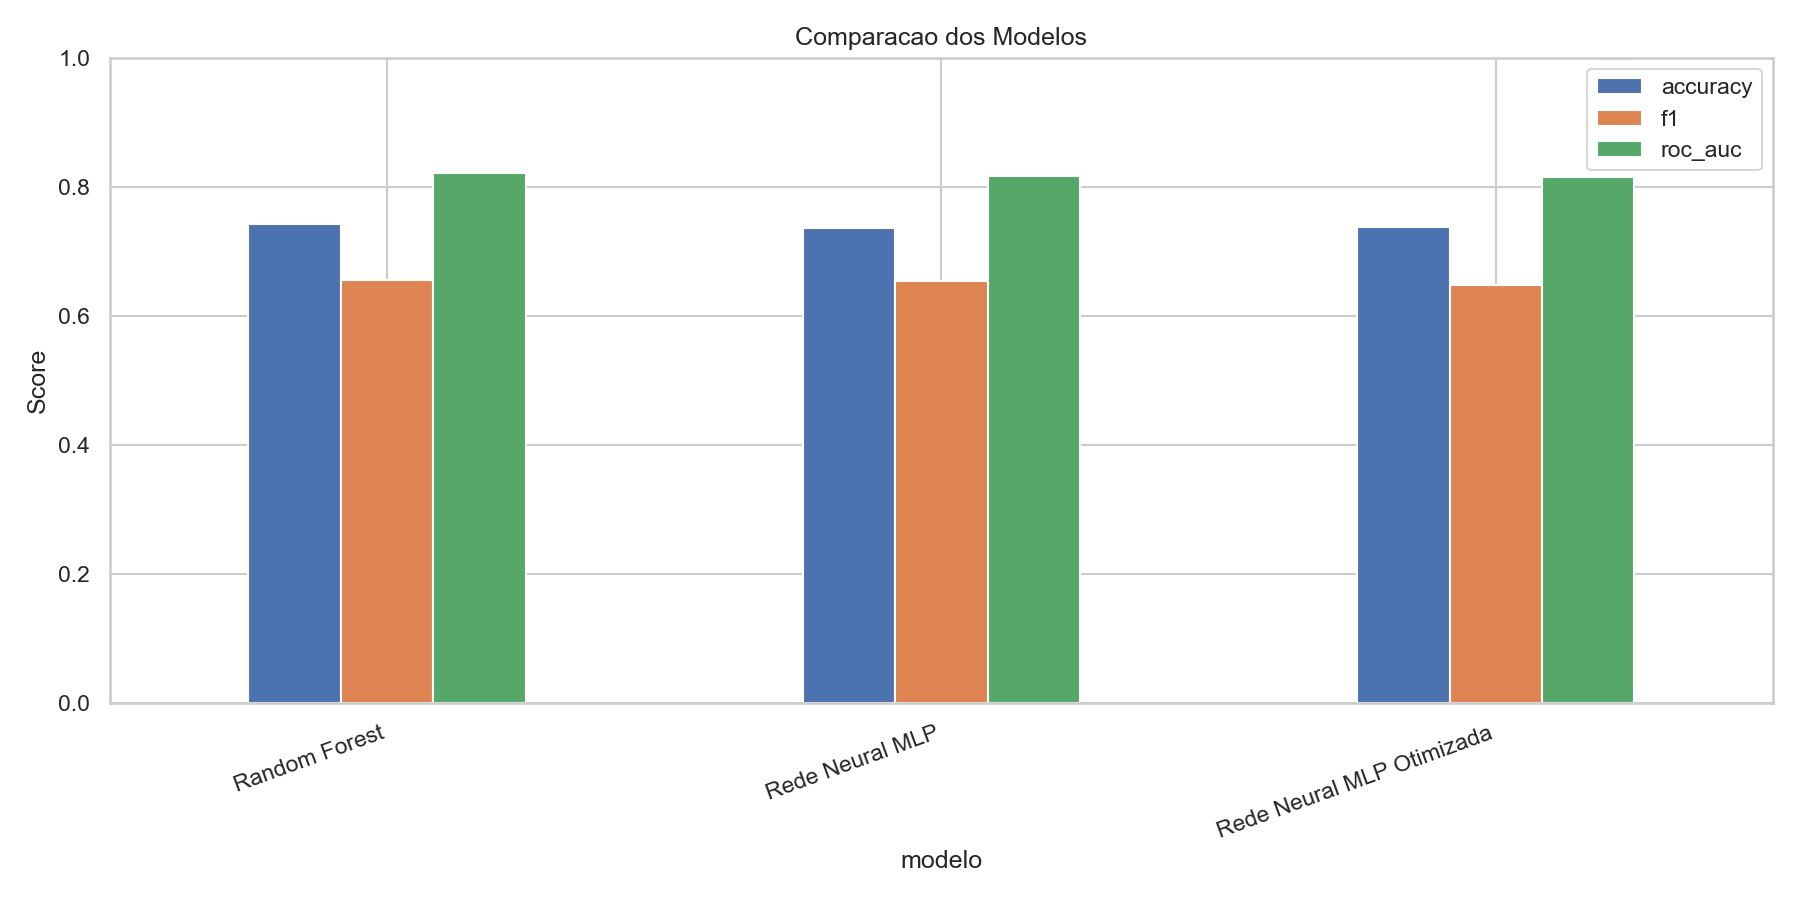
\includegraphics[width=\columnwidth]{notebook_model_comparison.png}
\caption{Visual comparison of performance metrics (Accuracy, F1-Score, and ROC AUC) across the three evaluated models: Random Forest, Baseline MLP, and Optimized MLP. The Random Forest leads uniformly across all three metrics.}
\label{fig:model_comparison}
\end{figure}

From a practical development standpoint, Random Forest also presented clear advantages over the neural network. The \texttt{GridSearchCV} with 12 hyperparameter combinations and 3 folds was executed on CPU in a reasonable time, without mandatory input normalization and with hyperparameters that have intuitive interpretations and predictable effects on performance. The neural network, in turn, demanded significantly more tuning effort: it was necessary to define the architecture (number of layers and neurons), learning rate, batch size, regularization strategy with Dropout and BatchNorm, and the EarlyStopping and ReduceLROnPlateau callbacks---in addition to continuous monitoring of training and validation curves to detect overfitting. The final result was that the optimized version of the network, despite all this additional tuning effort, achieved a gain of only 0.13 p.p.\ over its own baseline, reinforcing the diminishing returns of complexity in this specific problem.

Regarding interpretability, Random Forest holds a decisive advantage. Permutation importance, directly available through Scikit-learn, allows clear identification of which variables most influence the prediction, and the most important attributes---\texttt{sleep\_duration\_hrs}, \texttt{sleep\_quality\_score}, and \texttt{stress\_score}---are precisely those that the sleep medicine literature identifies as determinants of recovery quality \cite{hirshkowitz2015}, lending the model intuitive alignment with the domain. Each individual tree can also be visualized and its decision rules inspected. The neural network, by contrast, is essentially a black box: the weights distributed across multiple layers offer no direct explanation of decisions, and although techniques such as SHAP \cite{lundberg2017} can be applied \textit{a posteriori}, the interpretive cost is inherently higher.

Considering the identified trade-offs, Random Forest is preferable in scenarios with structured tabular data, tight deadlines, interpretability requirements, and predictive signal concentrated in few variables---situations where it is necessary to justify model decisions to non-technical stakeholders or comply with regulatory requirements such as algorithmic auditability standards in healthcare. Neural networks, on the other hand, become the more appropriate choice when data is high-dimensional with spatial or temporal structure (images, audio, time series, text), when the data volume is very large (in the order of millions of samples), when GPU computational resources are available for architectural exploration, or when the task involves learning complex hierarchical representations or transfer learning.

Among the main challenges encountered throughout the project, the first is the interpretation of metrics under class imbalance: the 61\% naive baseline forced the analysis to be guided by ROC AUC, Balanced Accuracy, and F1-Score, metrics that are less intuitive for communication with non-specialists. Another significant challenge was the predictability ceiling: both models converged to similar performance (${\sim}74\%$ accuracy), suggesting that the practical limit of the dataset had been reached---a diagnosis confirmed by the feature importance analysis, which revealed that the vast majority of variables contribute little information. The subjectivity of the \texttt{felt\_rested} target, as discussed, introduces irreducible ambiguity that no model can overcome. The neural network hyperparameter tuning also consumed multiple manual search iterations; a more systematic approach such as Optuna or KerasTuner could have explored the search space more efficiently within the available time. Finally, the hardware limitation---with training performed exclusively on CPU---restricted the speed of experimentation, particularly for wider architectures and more epochs, and the synthetic nature of the dataset, although calibrated with real correlations, may not capture all the non-linearities and confounders present in authentic population data, limiting the generalizability of the models to real clinical populations.

% -------------------------------------------------------
\section{Conclusion}

This work empirically demonstrated that, for the problem of classifying perceived sleep quality in a structured tabular dataset, Random Forest outperformed the MLP Neural Network across all evaluated metrics, with an Accuracy of 74.15\% and a ROC AUC of 0.8218. The most important conclusion of the experiment is not merely that Random Forest won by a small margin, but rather that the superiority of a model depends fundamentally on the nature of the problem. Neural networks are not automatically better---they excel in tasks with high-dimensional data, hierarchical structure, and large volumes. In tabular data with signal concentrated in few variables and a subjective target, tree-based models offer equal or superior performance with lower tuning cost and greater interpretability.

As future work, it is recommended to apply threshold adjustment techniques to maximize Recall, given the clinical context where False Negatives are more costly; to use SHAP for explainability analysis of the Random Forest; to evaluate the alternative target \texttt{sleep\_disorder\_risk} (multiclass), which may present greater discriminative power; and to validate the models on datasets with real actigraphy and polysomnography data.

% -------------------------------------------------------
\begin{thebibliography}{00}

\bibitem{walker2017}
M. Walker, \textit{Why We Sleep: Unlocking the Power of Sleep and Dreams}. New York: Scribner, 2017.

\bibitem{shu2020}
L. Shu, et al., ``Wearable emotion recognition using heart rate data from a smart bracelet,'' \textit{Sensors}, vol. 20, no. 3, p. 718, 2020.

\bibitem{breiman2001}
L. Breiman, ``Random forests,'' \textit{Machine Learning}, vol. 45, no. 1, pp. 5--32, 2001.

\bibitem{goodfellow2016}
I. Goodfellow, Y. Bengio, and A. Courville, \textit{Deep Learning}. Cambridge, MA: MIT Press, 2016.

\bibitem{dataset2024}
M. K. Thalla, ``Sleep Health and Daily Performance Dataset,'' Kaggle, 2024. [Online]. Available: \url{https://www.kaggle.com/datasets/mohankrishnathalla/sleep-health-and-daily-performance-dataset}

\bibitem{sklearn2011}
F. Pedregosa et al., ``Scikit-learn: Machine learning in Python,'' \textit{Journal of Machine Learning Research}, vol. 12, pp. 2825--2830, 2011.

\bibitem{chollet2015}
F. Chollet et al., ``Keras,'' GitHub, 2015. [Online]. Available: \url{https://keras.io}

\bibitem{grinsztajn2022}
L. Grinsztajn, E. Oyallon, and G. Varoquaux, ``Why tree-based models still outperform deep learning on tabular data,'' in \textit{Advances in Neural Information Processing Systems (NeurIPS)}, vol. 35, 2022, pp. 507--520.

\bibitem{hirshkowitz2015}
M. Hirshkowitz et al., ``National Sleep Foundation's sleep time duration recommendations: methodology and results summary,'' \textit{Sleep Health}, vol. 1, no. 1, pp. 40--43, 2015.

\bibitem{lundberg2017}
S. M. Lundberg and S.-I. Lee, ``A unified approach to interpreting model predictions,'' in \textit{Advances in Neural Information Processing Systems (NeurIPS)}, 2017, pp. 4765--4774.

\end{thebibliography}

\end{document}
